\documentclass{standalone}

\usepackage{pgfplots,mathtools}
\pgfplotsset{compat=newest}

\let\Re\relax
\DeclareMathOperator{\Re}{Re}
\let\Im\relax
\DeclareMathOperator{\Im}{Im}

\begin{document}
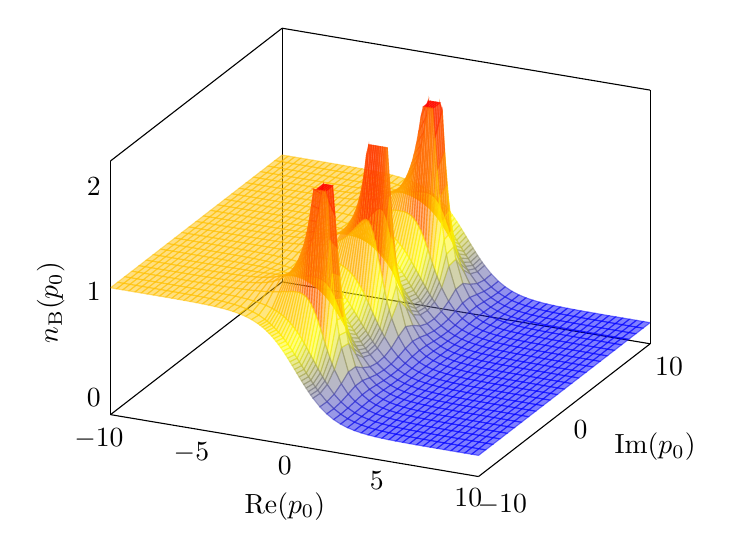
\begin{tikzpicture}
  \begin{axis}[
      xlabel=$\Re(p_0)$,
      ylabel=$\Im(p_0)$,
      zlabel=$n_\text{B}(p_0)$,
      x label style={at={(0.35, 0)}},
      y label style={at={(0.95, 0.15)}},
      shader=flat,
      tickwidth=0pt
    ]

    \def\nB{(e^(2*x) - 2*e^x*cos(deg(y)) + 1)^(-1/2)}

    \addplot3[surf, opacity=0.5, domain=1:10, y domain=-10:10]{\nB};

    \addplot3[surf, opacity=0.5, domain=-10:-2, y domain=-10:10]{\nB};

    \addplot3[surf, opacity=0.5, domain=-2:1, y domain=-10:10, restrict z to domain*=0:2]{\nB};

  \end{axis}
\end{tikzpicture}
\end{document}
